\documentclass[11pt]{beamer} % Options: handout = overlays aplatis a la compilation
%\usetheme{Berkeley}
\usetheme{Darmstadt}
\usecolortheme{crane}
%\usetheme{Bergen}

\usepackage[utf8]{inputenc}
\usepackage[english]{babel}
\usepackage[T1]{fontenc}
\usepackage{amsmath}
\usepackage{amsfonts}
\usepackage{amssymb}
\usepackage{graphicx}
\author{L. Charleux}
\title{ Des présentations avec Beamer}
%\setbeamercovered{transparent} 
%\setbeamertemplate{navigation symbols}{} 
%\logo{} 
\institute{USMB} 
\date{02 juin 2020} 
\subject{Une alternative à PowerPoint ?} 
\setbeamercovered{transparent} % Ce qui est caché est grisé

\begin{document}

\begin{frame}
\titlepage
\end{frame}

\begin{frame}
\tableofcontents
\end{frame}

\section{Introduction}
\begin{frame}{Beamer: c'est comme \LaTeX ?}
\begin{block}{Un bloc !}
$$
u = \int_0^{+\infty}v + \sum_0^{N-1} w
$$
\end{block}

\begin{alertblock}{Un alertbloc !}
\begin{itemize}
\item Truc
\item Bidule
\end{itemize}
\end{alertblock}

\begin{alertblock}{Enumerate}
\begin{enumerate}
\item Truc
\item Bidule
\end{enumerate}

\end{alertblock}

\end{frame}

\section{Les colonnes}

\begin{frame}{Les colonnes: une structure utile}
  \begin{columns}[c] % On démarre des colonnes centrées "c"
    \column{.5\textwidth} % On démarre une colonne de 50% de la largeur du texte dans le transparent
    	
    	\centering{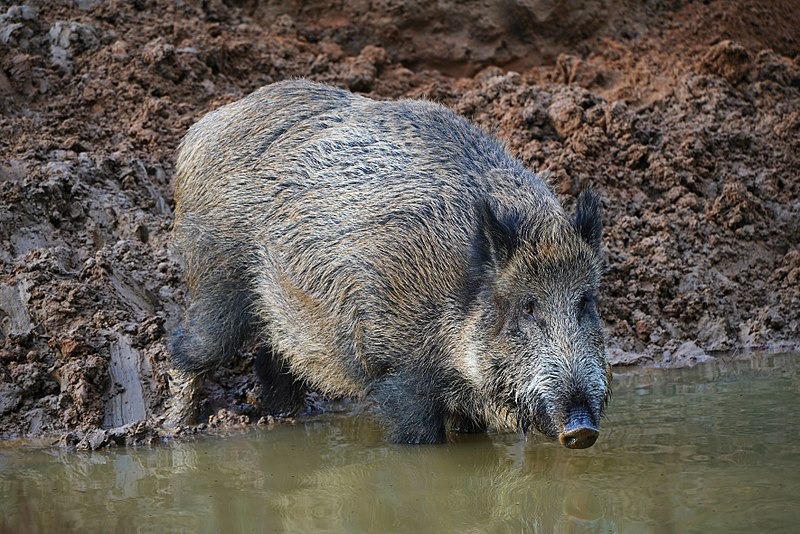
\includegraphics[width = 1\textwidth]{figures/boar.jpg}}
    \column{.5\textwidth} % On démarre une colonne de 50% de la largeur du texte dans le transparent
    	\begin{block}{Le sanglier}
    		\begin{enumerate}
    			\item Gros
    			\item Poilu
    			\item Un peu laid
    		\end{enumerate}
    	\end{block}
  \end{columns}
\end{frame}

\section{Les overlays}
\subsection{Les sangliers}

\begin{frame}{Rien}

\end{frame}

\begin{frame}{Animer avec des overlays}
  \begin{columns}[c] % On démarre des colonnes centrées "c"
    \column{.5\textwidth} % On démarre une colonne de 50% de la largeur du texte dans le transparent
    	
    	\centering{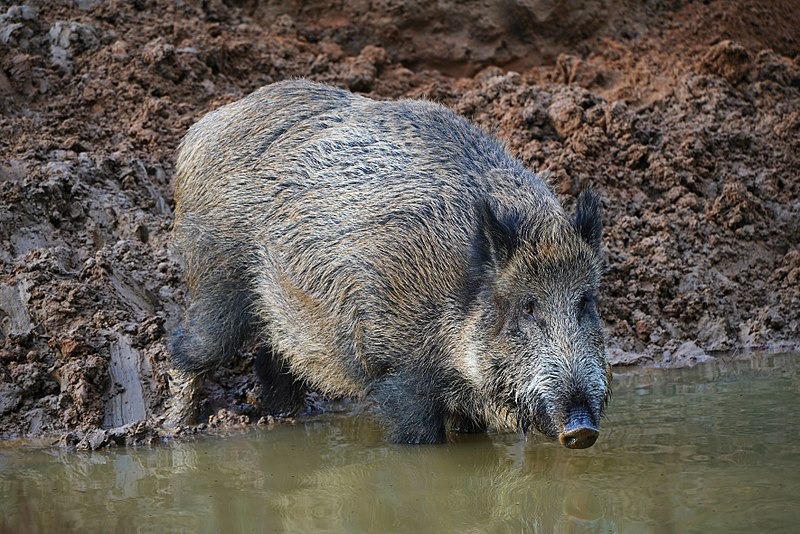
\includegraphics[width = 1\textwidth]{figures/boar.jpg}}
    \column{.5\textwidth} % On démarre une colonne de 50% de la largeur du texte dans le transparent
    	\begin{block}{Le sanglier}
    		\begin{enumerate}
    			\item<1-> Gros
    			\item<2-> Poilu
    			\item<3-> Un peu laid
    		\end{enumerate}
    	\end{block}
  \end{columns}
%  \only<4>{  
%    \begin{alertblock}{Conclusion}
%       C'est un badass !
%    \end{alertblock}
%  }
    \onslide<4>{  % Pareil que \only mais ça reserve la place.
    \begin{alertblock}{Conclusion}
       C'est un badass !
    \end{alertblock}
   } 
\end{frame}

\begin{frame}{Animer avec des overlays}
  \begin{columns}[c] % On démarre des colonnes centrées "c"
    \column{.5\textwidth} % On démarre une colonne de 50% de la largeur du texte dans le transparent
    	
    	\centering{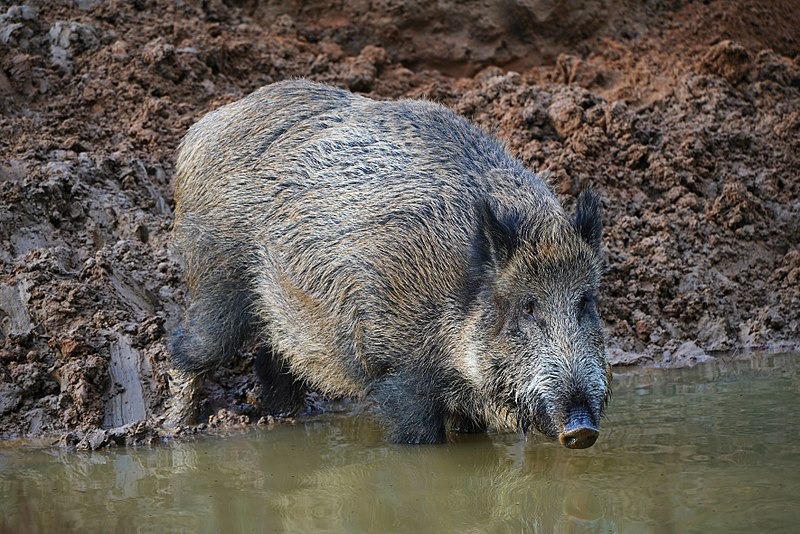
\includegraphics[width = 1\textwidth]{figures/boar.jpg}}
    \column{.5\textwidth} % On démarre une colonne de 50% de la largeur du texte dans le transparent
    	\begin{block}{Le sanglier}
    		\begin{enumerate}
    			\item<+> Gros
				\item<+> Sauvage !    			
    			\item<+-> Poilu
    			\item<+> Un peu laid
    		\end{enumerate}
    	\end{block}
  \end{columns}
%  \only<4>{  
%    \begin{alertblock}{Conclusion}
%       C'est un badass !
%    \end{alertblock}
%  }
    \onslide<4>{  % Pareil que \only mais ça reserve la place.
    \begin{alertblock}{Conclusion}
       C'est un badass !
    \end{alertblock}
   } 
\end{frame}

\end{document}